\ifx\allfiles\undefined
\documentclass[12pt]{book}
\usepackage[a4paper]{geometry}
\usepackage[dvipsnames]{xcolor}
\usepackage{amsmath, amsthm, amssymb, mathrsfs}
\usepackage{graphicx}
\usepackage{enumitem}

\usepackage{tikz}
\usepackage[colorlinks,linkcolor=black]{hyperref}
%\usepackage{biblatex}

\pagestyle{plain}

\graphicspath{ {fig/},{../fig/}, {config/}, {../config/} }

\geometry{top=25.4mm,bottom=25.4mm,left=20mm,right=20mm,headheight=2.17cm,headsep=4mm,footskip=12mm}
\linespread{1.5}
\setenumerate[1]{itemsep=5pt,partopsep=0pt,parsep=\parskip,topsep=5pt}
\setitemize[1]{itemsep=5pt,partopsep=0pt,parsep=\parskip,topsep=5pt}
\setdescription{itemsep=5pt,partopsep=0pt,parsep=\parskip,topsep=5pt}

% Theorem environment
\newtheorem{defn}{Definition}[section]

\newtheorem{lemma}{Lemma}[section]
\newtheorem{theorem}[lemma]{Theorem}
\newtheorem{corollary}[lemma]{Corollary}
\newtheorem{criterion}[lemma]{Criterion}

\newtheorem{proposition}{Proposition}[section]
\newtheorem{example}{Example}[section]
\newtheorem*{rmk}{Remark}


\def\d{\textup{d}}
\begin{document}
% \title{{\Huge Lecture-Notes on \\ \textbf{
Computational Methods in Evolutionary Biology}}}
\author{Chang Longxiao\\
longxiao.chang@campus.lmu.de}
\date{\today}

\maketitle                   % title in a newpage

\thispagestyle{empty}        % without page number
\begin{center}
    \Huge\textbf{FOREWORD}
\end{center}

"\textit{Nothing in biology makes sense except in the light of evolution}," said Theodosius Dobzhansky. Likewise, we could say that \textit{nothing in evolution makes sense except in the light of mathematics}.

As a child, I was fascinated by the vivid beauty of nature. As I grew older, this fascination led me to biology—the science that seeks to describe the dynamics of the living world. However, such descriptions often feel too imprecise, if not unscientific, to truly grasp the complexities of reality. Contrary to what many experimental biologists believe, There is too less mathematic languages used in biology, not too much.
%biology does not suffer from an excess of mathematics, but rather from a shortage of it.

Evolution, as the most fundamental and important topic in biology, appears to have the clearest structure that can be described mathematically, largely due to its long time scale. This note serves as a record of the models and methods I have learned in evolutionary biology. By building upon previous research, we may one day uncover a deeper understanding of the intricate complexity of life.

\begin{flushright}
    \begin{tabular}{c}
        \today \\ 
        Im Biozentrum LMU
    \end{tabular}
\end{flushright}

\iffalse
\begin{center}
    If people do not believe that mathematics is simple,

    it is only because they do not realize how complicated life is. 
    
    ——John von Neumann
\end{center}
\fi

\newpage                   
\pagestyle{plain}             
\setcounter{page}{1}          
\pagenumbering{Roman}    

\tableofcontents              

\newpage                   
\pagestyle{plain}
\setcounter{page}{1}          
\pagenumbering{arabic} 
\else
\fi

\chapter{Basics}

\section{Wright-Fisher Model and Kingman's Coalesce}
    \subsection{W-F model}
        \textbf{Basic assumptions of the Wright Fisher model}
        \begin{itemize}
            \item non-overlapping generations 
            \item constant population size
            \item panmictic
            \item neutral (i.e. no selection)
            \item no recombination
            \item $N$ diploid individuals population of $2N$ haploid alleles 
            
            (in case of autosomal DNA)
        \end{itemize}

        Each allele chooses an ancestor in the generation before. A population of $10$ individuals can be modeled as the figure.

        \begin{figure}[htbp]
            \centering
            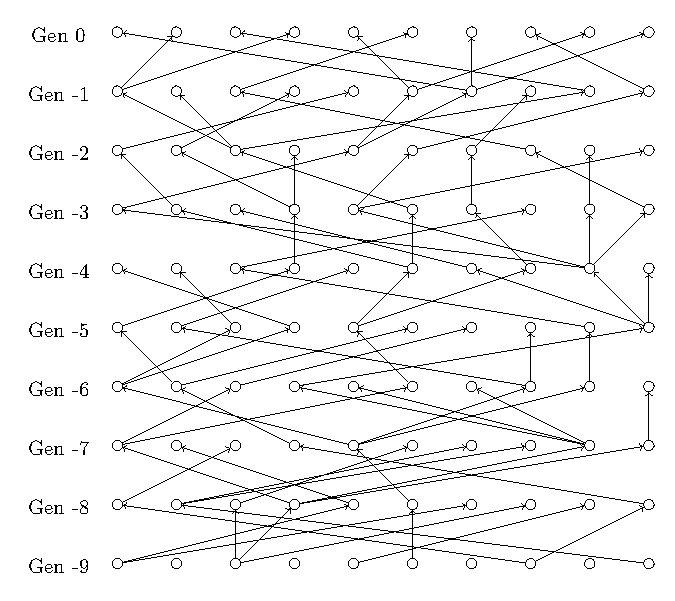
\includegraphics[scale = 1]{fig/W-F_123.pdf}
            \caption{simulated W-F model with $10$ individual and trace back $9$ generations}
        \end{figure}

        Samples are assumed to be taken purely randomly from the population. We take a sample of $4$ individuals from the population, for example, $(x,y,z,w)$.  
        \begin{figure}[htbp]
            \centering
            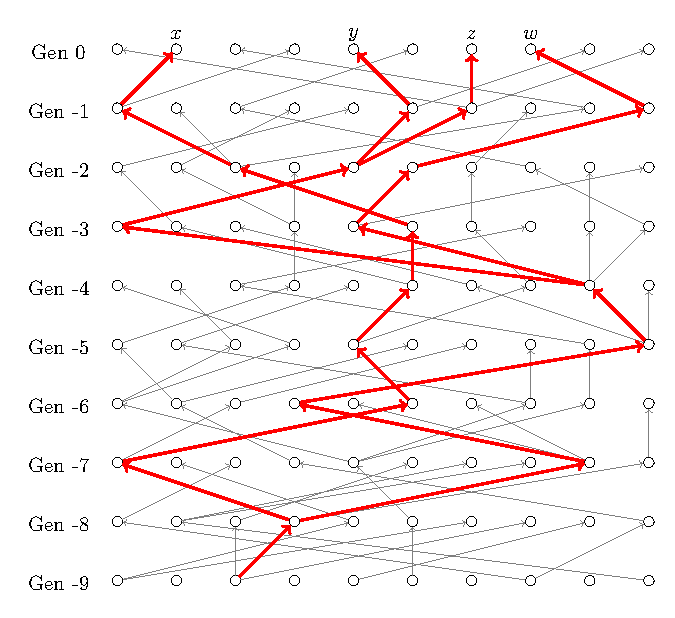
\includegraphics[scale = 1]{fig/W-F_123_label.pdf}
            \caption{simulated W-F population}
        \end{figure}

        Another simulation and sample.
        \begin{figure}[htbp]
            \centering
            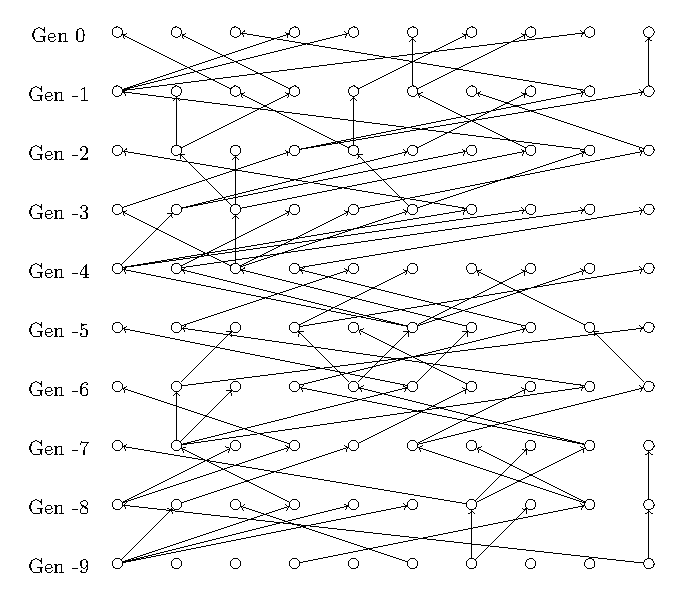
\includegraphics[scale = 0.55]{fig/W-F_888.pdf}
            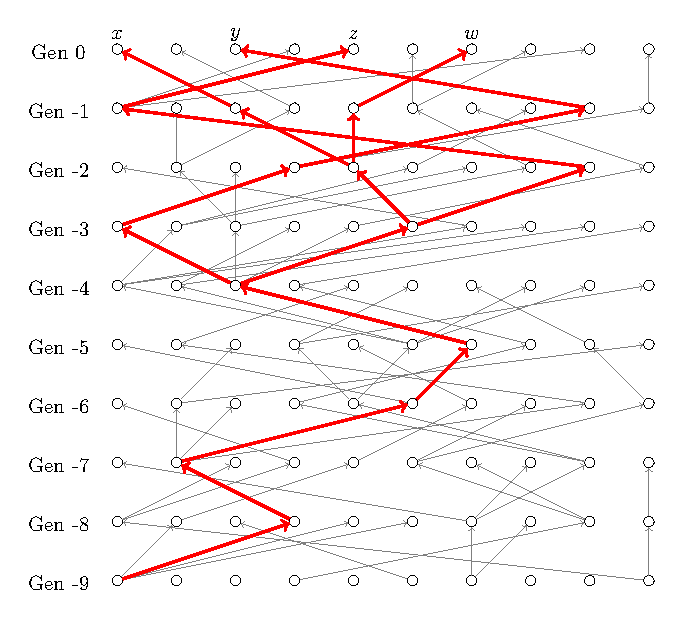
\includegraphics[scale = 0.55]{fig/W-F_888_label.pdf}
            \caption{simulated W-F population}
        \end{figure}

        This induces a specific random distribution for the genealogies of the sampled alleles.

        \begin{figure}[htbp]
            \centering
            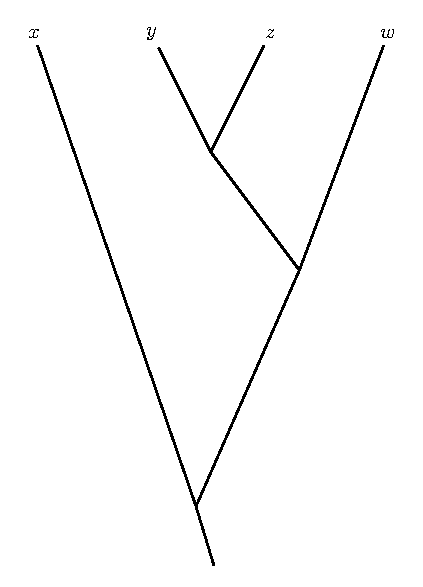
\includegraphics[scale = 0.8]{fig/W-F_result_123.pdf}
            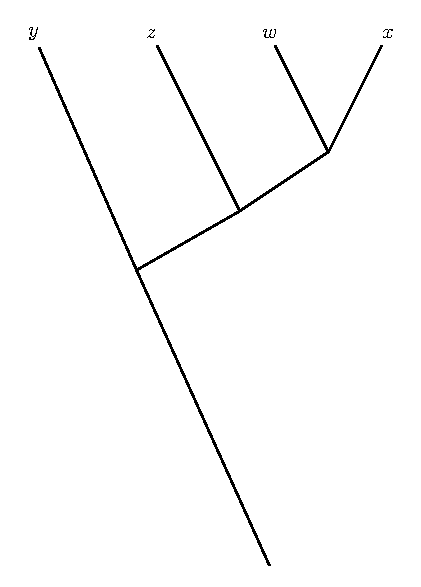
\includegraphics[scale = 0.8]{fig/W-F_result_888.pdf}
            \caption{simulated W-F population}
        \end{figure}
        
        Haploid population of size $N_e$


\ifx\allfiles\undefined
\end{document}
\fi